\documentclass{article}

\usepackage{multicol}
\usepackage{titlesec}
\usepackage{graphicx}
\usepackage{wrapfig}
\usepackage{hyperref}
\usepackage{float}

\graphicspath{{./images/}}

\begin{document}

\title{RP2040 MACROPAD}
\author{Anna Denisova\\SNC1W\\Dr. Zehra\\March 2023}
\date{}

\maketitle

\tableofcontents

\newpage

\section{Abstract}

\hspace{1cm} This project explores the use of the RP2040 Macropad to create a digital musical instrument. The possibility of combining and incorporating both software and hardware aspects of technology is tested, making this an opportunity to learn about programming, electronics, and music all at once. The RP2040 Macropad is implemented in a way which 12 keys are used to control different note pitches in a given octave. The octave itself can be increased or decreased using the rotary encoder. When a key is pressed, its note and octave value is printed to the screen of the connected laptop/computer. For convenience, there are also buttons to print newlines and sound the whole scale of the selected octave at once. This project was chosen because it has many real world applications. It can be used as an educational tool that helps users learn the fundamentals of music theory. Also, it can be used as a device to help with tuning where users can compare real life sounds to the sounds outputted by a computer to determine accuracy. Overall, the RP2040 was successfully coded with software that works as intended.

\section{Introduction \& Objective}

\hspace{1cm} The RP2040 Macropad is a powerful and versatile device that can be coded in different programming languages to perform a wide range of functions. It is based on the high performance RP2040 microcontroller chip designed by Raspberry Pi. It has a large chip memory, a symmetric dual-core processor complex, deterministic bus fabric, and a rich peripheral set [1]. The Macropad itself comes with twelve keys, a rotary encoder and an OLED screen. In this project, we explore its capabilities using the Arduino IDE and C++ to create useful software. 

\section{Purpose}

The purpose of this project is to create software for the RP2040 Macropad to play notes of different octaves using the built in speaker. 

\section{Hypothesis}

If I write specific code for the RP2040 Macropad, then I can output different sound frequencies because of the software created.

\newpage
\section{Variables}

\underline{Control}
\begin{itemize}
    \item The RP2040 Macropad
    \item Additional buttons with fixed functionalities
    \item Computer, USB cord
\end{itemize}
\underline{Dependent}
\begin{itemize}
    \item Musical tone produced when a key is pressed (dependent on note pitch assigned to the key and the current octave set by the rotary encoder)
    \item The note names printed to the computer screen (depend on key pressed)
\end{itemize}
\underline{Independent}
\begin{itemize}
    \item Note pitches assigned to each key on the MacroPad
    \item The rotary encoder as it can be turned to change the octave value
\end{itemize}

\section{Materials}

\begin{itemize}
    \item Full kit with all parts found here: https://www.adafruit.com/product/5128 or alternatively:
    \item
        \begin{itemize}
            \item 3x4 keys
            \item Encoder
            \item OLED display
            \item 12 mechanical key switches
            \item 12 keycaps
            \item Adafruit MacroPad bottom plate
            \item 3x4 mechanical keyboard plate
            \item D-Shaft skirted rubber knob
            \item 4 M3 5mm machine screw
            \item 4 rubber feet
        \end{itemize}
    \item MacOS computer/laptop
    \item USB cable
\end{itemize}

\newpage
\section{Procedure}

\begin{enumerate}
    \item Set up your development environment (Arduino IDE) with the necessary tools to program your RP2040 Macropad.
    \begin{enumerate}
        \item Download the latest version of the Arduino IDE.
        \item Add the Philhower Board Manager URL to download additional boards including the RP2040 Macropad.
        \item In the Arduino IDE, go to Tools \textgreater{} Board \textgreater{} Boards Manager to select the RP2040 Macropad. 
        \item In the Sketch Tab, go to Port and select the corresponding port of the board.
        \item Now, the IDE is all set for code to be written in and run.
        \item Connect the board to your computer via USB.
        \item The board itself can  be reset by pressing the reset button on the edge of it.
        \item To enter the bootloader, press the rotary encoder and while continuing holding it down, press and release the reset button. Continue holding the rotary encoder down until the RPI-RP2 drive appears on your computer. 
    \end{enumerate}

    \item No, you are all set to write C++ code.
    
    \item Define the notes and their corresponding frequencies using a lookup table. Some of these tables can be found here:
    \begin{itemize}
        \item \url{https://pages.mtu.edu/~suits/notefreqs.html}
        \item \url{https://mixbutton.com/mixing-articles/music-note-to-frequency-chart/}
        \item \url{https://en.wikipedia.org/wiki/Piano_key_frequencies}
        \item \url{https://www.liutaiomottola.com/formulae/freqtab.htm}
    \end{itemize}
    
    \item Define key-to-note mapping using an array, if statements, or a switch statement.

    \item Code the rotary encoder to deal with octave values. With each step to the right (clockwise) on the rotary encoder, increase the octal value.
    
    \item When a key is pressed, call the tone() function to play the note through the speaker. 

    \item Finally, allow printing to the computer so that the note values are outputted on the computer screen when active in any text editor (notepad, word, docs, etc.)

    \item Set up any additional buttons with any additional functions. 

    \item Compile and upload the code to the RP2040 Macropad. 
        
   
\end{enumerate}

\section{Safety Precautions}
\begin{itemize}
    \item Properly handle electrical components so as to not damage them or produce any electric shock
    \item Have the correct connections throughout the device before applying power to prevent shorts or other issues
    \item Be mindful of heat being generated by the components
    \item Use proper documentation of the circuit and code
    \item Follow other various best practices
\end{itemize}

\section{Experiment - The build}

\hspace{1cm} With a pre-bought RP2040 Macropad kit, the assembly was fairly quick and straightforward. The two most popular and convenient options for which language to use in code are Python and C++. In this specific building process, C++ was used.\\\\

The board itself was coded over a span of three days with base code to go off of. First, the pitches were assigned to each key with the rotary encoder set to change the octaves. Then, using the "Keyboard.h" library, the functionality of printing the note names to the computer was added. The additional buttons were then coded with more functionalities like adding a newline and playing the notes of a specific octave at once. \\\\

At times, the board had to be unplugged to cool off because of excessive usage causing it to heat up. Testing was a very crucial part as well. As new functions were added, testing was necessary to confirm the correctness of newly added code. \\\\

Here is the final program:\\

\begin{figure}[H]
    \centering
    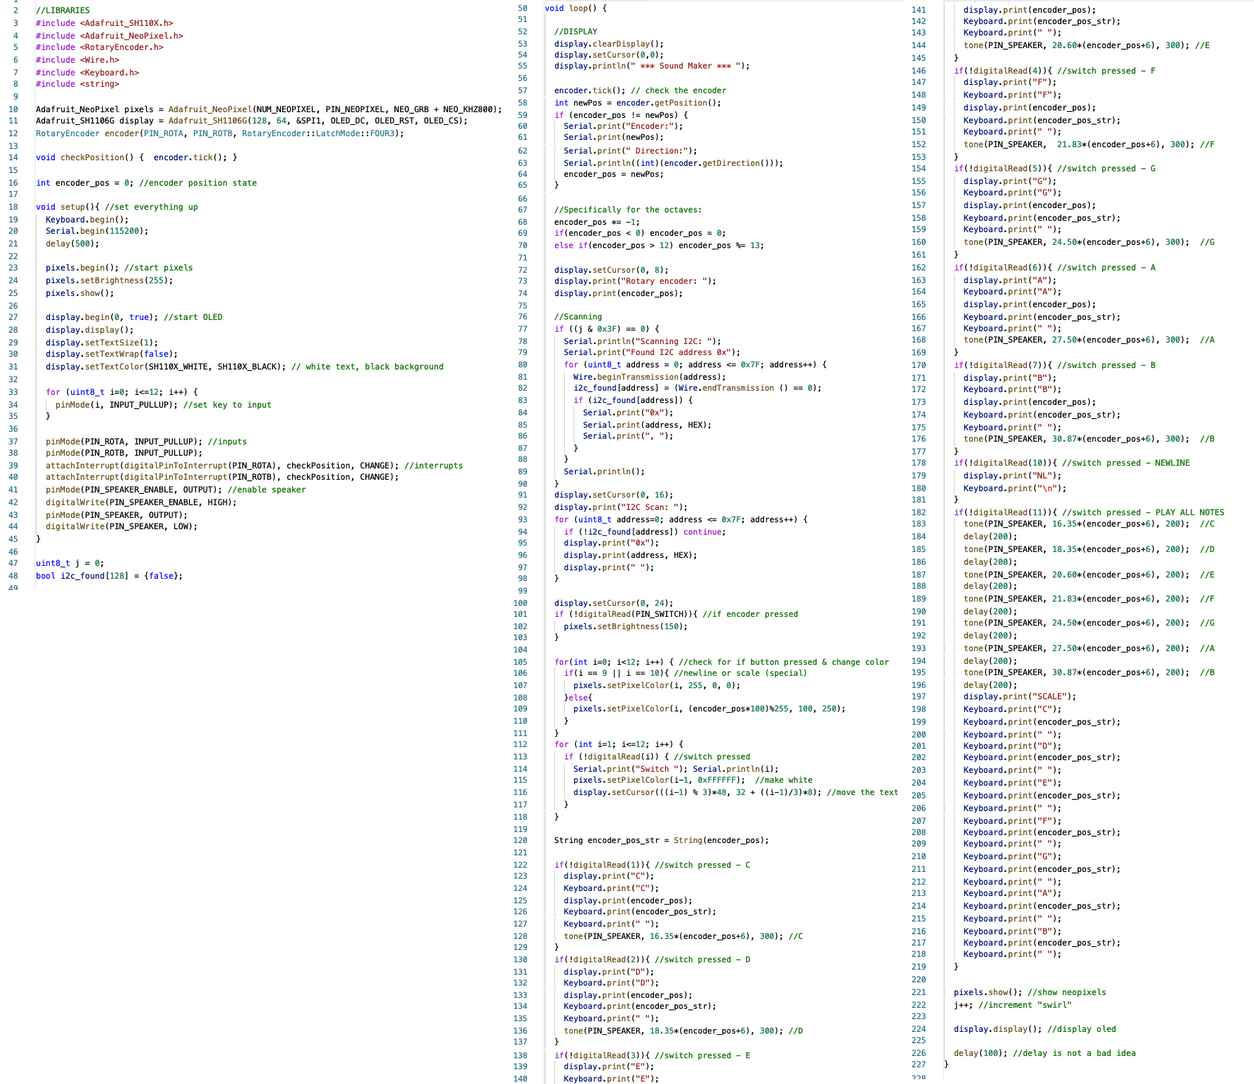
\includegraphics[width=\textwidth]{images/CODE.png}
\end{figure}

\noindent
\underline{Here are links to videos:}\\
The building process: \url{https://drive.google.com/file/d/1dza2j5ACgz4srzRRXTJErM3iTjd8o5mv/view?usp=share_link} \\
Playing a song: \url{https://drive.google.com/file/d/1CDH2NvlKspHmQtVSUsXAfAaJQbIO9Aq_/view?usp=share_link}\\

\section{Results \& Analysis}

\hspace{1cm} The creation process did not always run smoothly. Of course, there were bugs and some plans did not go as intended which forced specific functions to be redesigned and re-programmed. For example, I had to figure out how to map out the frequencies of waves to their corresponding note values and their octaves.\\\\

Generally, there were many different ways for going about how to design the program. There isn't always one specific way to achieve a function/task but rather an array of different options and paths to take. Of course, some paths may be more efficient and generally better in principle. \\\\

One of the biggest challenges was  fine-tuning each of the different functionalities coded. The tone generator had to produce the pitches at the correct frequencies for each octave, the position of the rotary encoder had to be carefully monitored and checked, and the structure of the code had to be logical and efficient. However, through testing and research, I was able to overcome these challenges. Overall, from a technical standpoint, the RP2040 Macropad is a well-designed and implemented project that demonstrates good understandings of hardware interfacing, software development, and embedded systems. The use of tone generation to produce different pitches and frequencies for each note and octave teaches the creator the underlying principles of sound generation and modulation.\\\\

\section{Conclusion \& Application}

\hspace{1cm} Using the built in speaker, a program was created to map the keys of the RP2040 Macropad to different musical notes with the rotary encoder making the octaves adjustable.\\\\

The RP2040 microcontroller chip designed by Raspberry Pi has high performance, a low cost, and flexible I/O. It can communicate with almost any external device making it very useful in real life applications [2]. In this project, the microcontroller is directly connected to an external laptop to transfer signals through a USB cable. \\\\

There are several practical applications for this project. One such application is an educational tool to help users learn the basics of music theory. Also, the RP2040 Macropad can be used as a tuning device, allowing users to compare real-life sounds to the computer-generated sounds in order to determine accuracy. The ability to print the note names to the computer screen and play the corresponding tones in real-time creates a compelling user experience. \\\\

Completing this project is a reliable way to gain educational experience and a deeper understanding of microcontrollers. Personally, I gained more experience with understanding the fundamentals of the RP2040. I learned how to program code for the buttons, rotary encoder, and tone generator. Also, I learned how to use many different code libraries such as the Adafruit NeoPixel library, the Rotary Encoder library and the Keyboard Library.\\\\

However, there are also many potential sources of error that may occur when developing such a project. There could be issues with signals which could lead to notes being off pitch or having inconsistent timing. The rotary and button errors may fail to register input correctly and there could also be communication issues when connecting the Macropad to the laptop/computer. Finally, the most common error that could occur is within the code. These include bugs, logic, or any syntax errors that could cause unexpected behavior or crashes. \\\\\

Of course, the abilities of the RP2040 Macropad do not end here. There are still many more different projects to create and experiment with!

\section{Libraries Used}

The code uses the following libraries: \\
\begin{itemize}

    \item \begin{verbatim}Adafruit_SH110X.h\end{verbatim} 
    Copyright (c) 2012, Adafruit Industries. All rights reserved. \\
    License: BSD

    \item \begin{verbatim}Adafruit_NeoPixel.h\end{verbatim} 
    Copyright (c) 2007,Free Software Foundation \\
    License: LGPL-3.0

    \item \begin{verbatim}RotaryEncoder.h\end{verbatim} 
    Copyright (c) 2005-2014 by Matthias Hertel,  http://www.mathertel.de/  \\
    License: BSD

    \item \begin{verbatim}Wire.h\end{verbatim} 
    Copyright (c) 2006 Nicholas Zambetti.  All right reserved. \\
    License: LGPL-3.0

    \item \begin{verbatim}Keyboard.h\end{verbatim} 
    Copyright (c) 2015, Arduino LLC \\
    License: LGPL-3.0

\end{itemize}


\section{Bibliography}

\begin{enumerate}
\item \url{https://datasheets.raspberrypi.com/rp2040/rp2040-product-brief.pdf}\\
\item \url{https://www.raspberrypi.com/products/rp2040/} \\
\item \url{https://www.adafruit.com/product/5128} \\
\item \url{https://learn.adafruit.com/adafruit-macropad-rp2040} \\
\item \url{https://cdn-learn.adafruit.com/downloads/pdf/adafruit-macropad-rp2040.pdf} \\
\item \url{https://www.arduino.cc/} \\ 
\item \url{https://pages.mtu.edu/~suits/notefreqs.html} \\
\item \url{https://mixbutton.com/mixing-articles/music-note-to-frequency-chart/} \\
\item \url{https://en.wikipedia.org/wiki/Piano_key_frequencies} \\
\item \url{https://www.liutaiomottola.com/formulae/freqtab.htm} \\
\end{enumerate}

%-------------------------------------------------------------------------------------------------------------


\end{document}